\documentclass[11pt]{ltjsarticle}
\usepackage{amsmath}
\usepackage{amssymb}
\usepackage{amsfonts}
\usepackage{physics}
\usepackage{graphicx}
\usepackage{float}
\usepackage{booktabs}
\usepackage{tikz}
\usepackage{xcolor}
\usepackage{pgfplots}
\usepackage{mathcomp}
\usepackage{enumitem}
\usepackage{wrapfig}
\usepackage{etoolbox}
\usepackage{cleveref}
\usepackage[version=4]{mhchem}
\crefformat{figure}{図~#2#1#3}  % 図の日本語設定
\crefformat{equation}{式~(#2#1#3)}  % 式の日本語設定
\crefformat{table}{表~#2#1#3}  % 表の日本語設定
\usetikzlibrary{intersections,calc}
\pgfplotsset{compat=1.18}
\begin{document}
\begin{figure}[H]
  \centering
  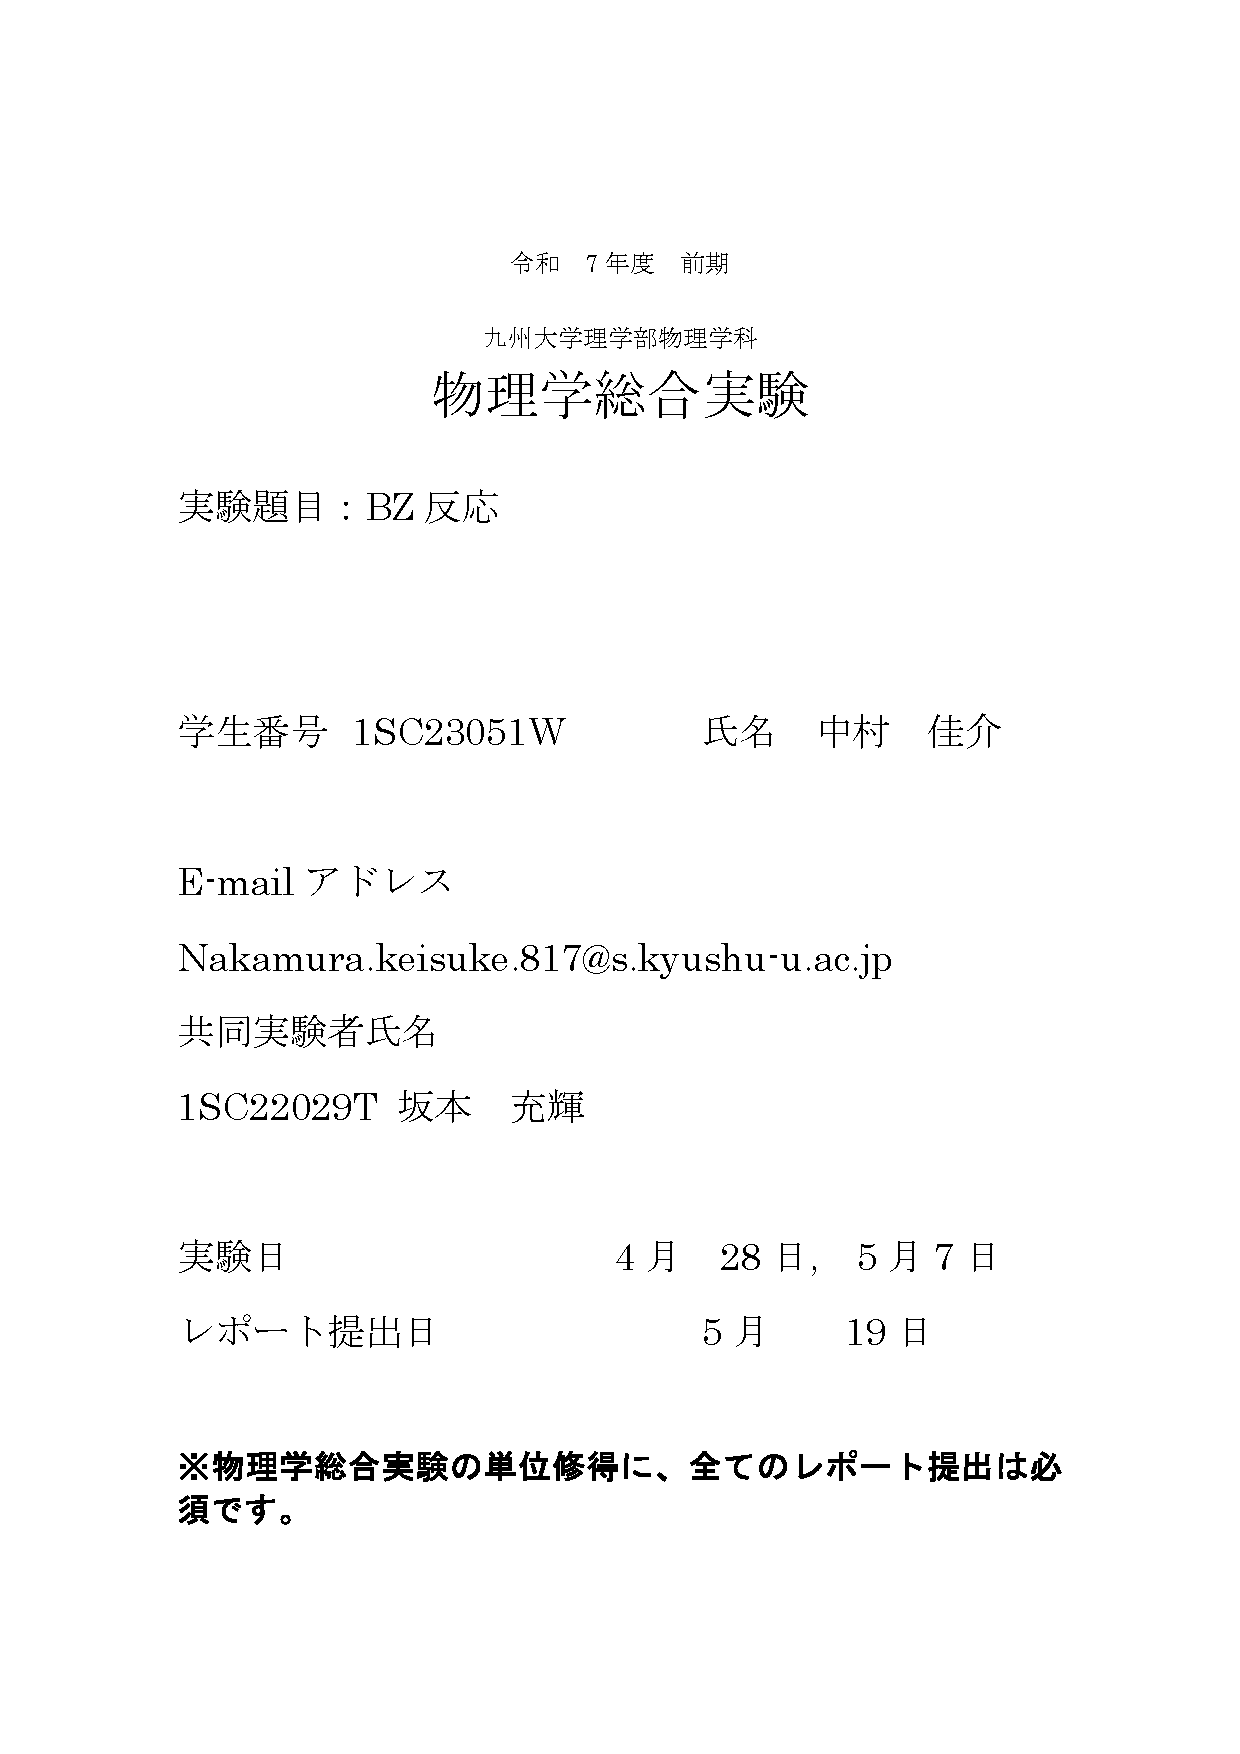
\includegraphics[width=0.98\columnwidth]{hyoushiBZ.pdf}
\end{figure}

  \section*{目的}
    溶液の色が時間的に振動するBZ反応について画像解析などを用いて理解する.
  \section*{原理}
    1951年, ロシアのBelousovが生物の代謝経路を模倣した化学反応系で実験を行ったところ, 溶液の色が時間的に振動することを発見したが, 当時の学会には受け入れられなかった.その後1964年にロシアのZhabotinskyによって再現され, この実験が正しいと認められることになった. この二人の名前をとってこの実験はBZ反応と呼ばれる. \\
    BZ反応はその反応が進んだり戻ったりするので, 熱力学に反しているように見えるがもちろんそんなことはなく, 反応を繰り返し(その結果として溶液の色が変化しながら)少しずつ平行に向かっているのである. \\
    BZ反応では溶液中の金属錯体イオンが酸化還元を繰り返し振動反応を繰り返す. よって今回の実験では酸化状態によって呈色する鉄イオンを用いた. 鉄イオンは2価と3価でそれぞれのフェナントロリン錯体がそれぞれ赤と青で呈色する. 
    \subsection*{反応モデル}
    BZ反応はその反応段階が多く複雑で詳細が明らかになるのに時間がかかった. BZ反応の研究の初期段階では振動するという条件を満たした数理モデルを実験と比較することで解析していた. 1972年にField, Körös, Noyesらにより反応段階がすべて解明され, FKNモデルと呼ばれるモデルが提唱された. 
    これは反応段階を10段以上に分けるものであり, 以下に本実験のFKNモデルの化学反応式を示している.
    \begin{gather}
      \ce{HBrO + Br^- + H+ <=> Br2 + H2O} \\
      \ce{HBrO2 + Br^- + H+ -> 2HBrO} \\
      \ce{BrO3^- + Br^- + 2H+ -> HBrO2 + HBrO} \\
      \ce{2HBrO2 -> BrO3^- + HBrO + H+} \\
      \ce{BrO3^- + HBrO2 + H+ <=> 2BrO2 + H2O} \\
      \ce{BrO2 + Fe^2+ + H+ <=> HBrO2 + Fe^3+} \\
      \ce{BrO2 + Fe^3+ + H2O -> BrO3^- + Fe^2+ + 2H+} \\
      \ce{Br2 + CH2(COOH)2 -> BrCH(COOH)2 + Br^- + H+} \\
      \ce{6Fe^3+ + CH2(COOH)2 + 2H2O -> 6Fe^2+ + HCOOH + 2CO2 + 6H+} \\
      \ce{4Fe^3+ + BrCH(COOH)2 + 2H2O -> Br^- + 4Fe^2+ + HCOOH + 2CO2 + 5H+}
    \end{gather}
    これから律速とならないものをまとめて5段階の反応にし, 時間変化が少ない変数を定数にして三変数の方程式にしたものがオレゴネータである.\\
    さらに変化速度が他に比べて速く, あまり変化しない変数を定数にした2変数オレゴネータと固定点周りの挙動が定性的に等しいフィッツフュー・南雲モデル(\cref{eq:nakumo1},\cref{eq:nakumo2})を今回用いた. 
    \begin{gather}
      \epsilon \qty(\frac{dx}{d\tau})=x-x^3-z
      \label{eq:nakumo1}\\
      \frac{dz}{d\tau}=ax-z
      \label{eq:nakumo2}
    \end{gather}
  \section*{実験}
    \subsection*{測定手順}
      \subsubsection*{ストック溶液の作成} 
      混合後の溶液の濃度がおおよそ\cref{tab:kongougo}になるようにストック溶液を以下の手順で濃く準備した. (M=mol/l)\\
      \begin{enumerate}
        \item 試薬の秤量:電子天秤を用いてあらかじめmol数と分子量から計算しておいた量を量り取った. (フェロイン溶液は1.10フェナントロリンと硫酸第一鉄(Ⅱ)モル比3:1で水に溶かす. )
        \item 作成する体積(100ml)の八割程度になるように純水を加え, ビーカー内でスターラーを用いて攪拌し, 溶解させた. この際, ラップで軽く蓋をして回転数を徐々に上げていった. 
        \item 完全に溶解したことを確認し, メスフラスコへ移し水を加えて標線に合わせた. (共洗いを三回以上行った.)
      \end{enumerate}
      結果的に用意したストック溶液の濃度は\cref{tab:stock}のようになった. 
      \begin{table}[H]
       \centering
        \begin{tabular}{lll}
          臭素酸ナトリウム & \ce{NaBrO3} & 0.15M \\
          臭化カリウム     & \ce{KBr} & 0.030M \\
          マロン酸         & \ce{CH2(COOH)2} & 0.10M \\
          硫酸             & \ce{H2SO4} & 0.60 \\
          フェロイン       & \ce{[Fe(C12H8N2)3]SO4} & 0.0050M \\
        \end{tabular}
        \caption{反応後の濃度}
        \label{tab:kongougo} 
      \end{table}
      \begin{table}[H]
        \centering
        \begin{tabular}{lll}
          臭素酸ナトリウム & \ce{NaBrO3} & 1.0M \\
          臭化カリウム     & \ce{KBr} & 0.30M \\
          マロン酸         & \ce{CH2(COOH)2} & 1.0M \\
          硫酸             & \ce{H2SO4} & 3.0M \\
          フェロイン       & \ce{[Fe(C12H8N2)3]SO4} & 0.050M \\
        \end{tabular}
        \caption{ストック溶液の濃度}
        \label{tab:stock} 
      \end{table}
      \subsubsection*{ビーカーでの時間変化}
      \begin{enumerate}
        \item ビーカーに臭素酸ナトリウム12ml, 臭化カリウム10ml, マロン酸12mlの順で入れた.
        \item ドラフトの中で1.を攪拌しながら硫酸13mlを加え, 溶液が完全に透明になるまで攪拌しつづけた.
        \item フェロイン0.6mlを入れ, 攪拌をつづけた. 
        \item BZ反応を観察, 記録した.
        \item 廃液はドラフト内に安置し, 実験終了後にポリタンクに入れ廃棄した.
      \end{enumerate}
      \subsubsection*{シャーレでの空間変化}
      \begin{enumerate}
        \item シャーレに蒸留水2.5ml, 臭素酸ナトリウム1.5ml, 臭化カリウム1.0ml, マロン酸1.0mlの順で入れた.
        \item ドラフトの中で攪拌しながらの硫酸3.0mlを加え, 溶液が完全に透明になるまで攪拌しつづけた.
        \item フェロイン1.0mlを入れ, 攪拌をつづけた. 
        \item BZ反応を観察, 記録した.
        \item 廃液はドラフト内に安置し, 実験終了後にポリタンクに入れ廃棄した.
      \end{enumerate}
  \section*{結果}
  輝度値を画像解析した結果が\cref{fig:beaker_Intensity}, \cref{fig:dish_Intensity}であり, ビーカーは時間的に, シャーレは空間的に振動していることがわかる. 
    \begin{figure}[H]
      \centering
      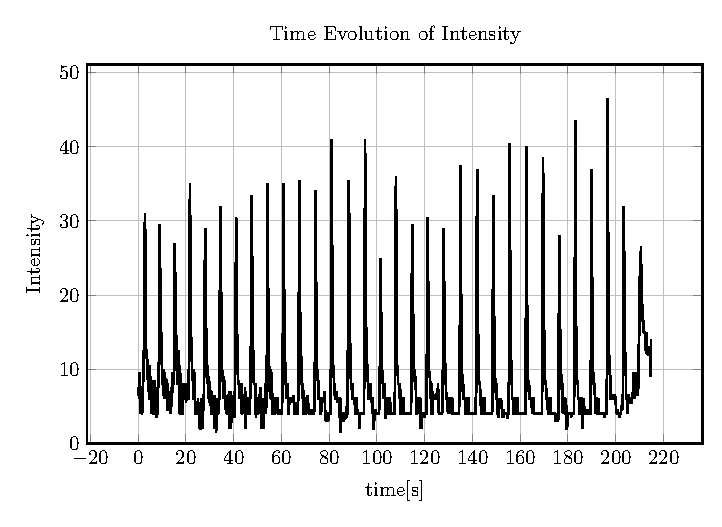
\includegraphics[width=0.7\columnwidth]{BZ_graph1.pdf}
      \caption{ビーカーの輝度値の時間変化}
      \label{fig:beaker_Intensity}
    \end{figure}
    \begin{figure}[H]
      \centering
      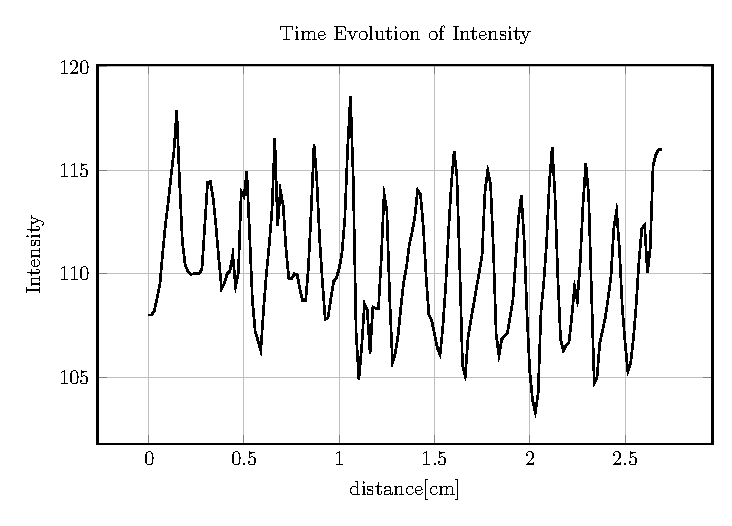
\includegraphics[width=0.7\columnwidth]{BZ_graph3.pdf}
      \caption{シャーレの輝度値の空間変化}
      \label{fig:dish_Intensity}
    \end{figure}
  \section*{考察}
    \subsection*{課題1}
      画像解析の結果は\cref{fig:beaker_Intensity}であり, 一定の周期で輝度値が変化し, 振動していることがわかる.また, フーリエ変換したパワースペクトルも最初の周波数から整数倍でパワースペクトルが立っており, フーリエ変換によって周期的に分解できていることがわかる.
      \begin{figure}[H]
        \centering
        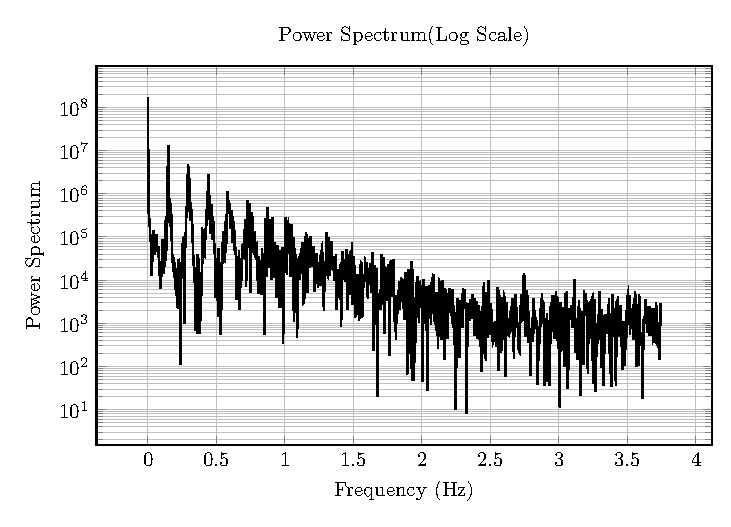
\includegraphics[width=0.7\columnwidth]{BZ_graph2.pdf}
        \caption{輝度値をフーリエ変換したパワースペクトラム(ビーカー)}
        \label{fig:beaker_power}
      \end{figure}
    \subsection*{課題2}
      画像解析の結果は\cref{fig:dish_Intensity}であり, こちらも一定の距離で輝度値が変化し, 振動しているように見える. フーリエ変換したパワースペクトルが\cref{fig:dish_power}であるが, ビーカーのグラフに比べ,一つの大きな周期があるのみで周期性は見られなかった. これは適切なフーリエ変換がされてないのが原因だと考えられる.
      \begin{figure}[H]
        \centering
        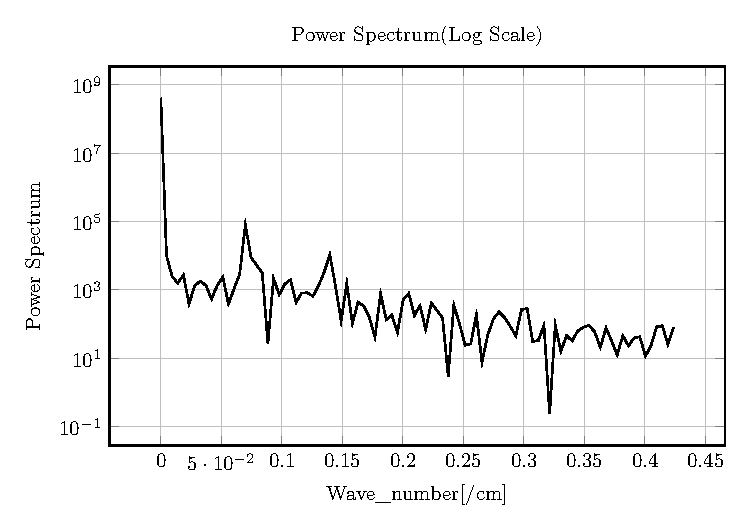
\includegraphics[width=0.7\columnwidth]{BZ_graph4.pdf}
        \caption{輝度値をフーリエ変換したパワースペクトラム(シャーレ)}
        \label{fig:dish_power}
      \end{figure}
    \subsection*{課題3}
      \subsubsection*{(i)}
        \cref{fig:nullcline}はフィッツフュー・南雲モデルのヌルクラインを示している. ヌルクラインは\cref{eq:nakumo1}, \cref{eq:nakumo2}の右辺が0になるような点を結んだものである. これは定常状態を示しており, 定常状態では時間変化がないことを示している. また, a=1とした.
        \begin{figure}[H]
          \centering
          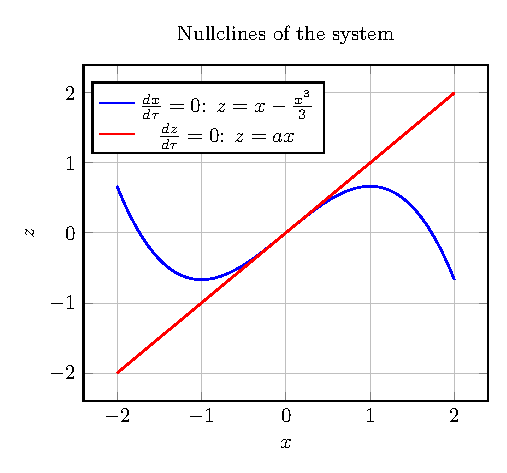
\includegraphics[width=0.7\columnwidth]{BZ_graph5.pdf}
          \caption{フィッツフュー・南雲モデルのヌルクライン}
          \label{fig:nullcline}
        \end{figure}
      \subsubsection*{(ii),(iii)}
      \cref{fig:phase1}は左側がa=1.0, 右側がa=0.1のときのフィッツフュー・南雲モデルの相図を示している.向きを矢印で, 大きさを色で表した.
        \begin{figure}[H]
          \raggedleft
          \includegraphics[width=0.98\columnwidth]{BZ_graph6.pdf}
          \caption{\epsilon=0.01のときの相図}
          \label{fig:phase1} 
        \end{figure}
    \subsection*{課題4}
      \subsubsection*{(i)}
        a,\epsilon,初期値それぞれを二パターンの値で計算した結果のグラフを以下に示す.
        \begin{figure}[H]
          \centering
          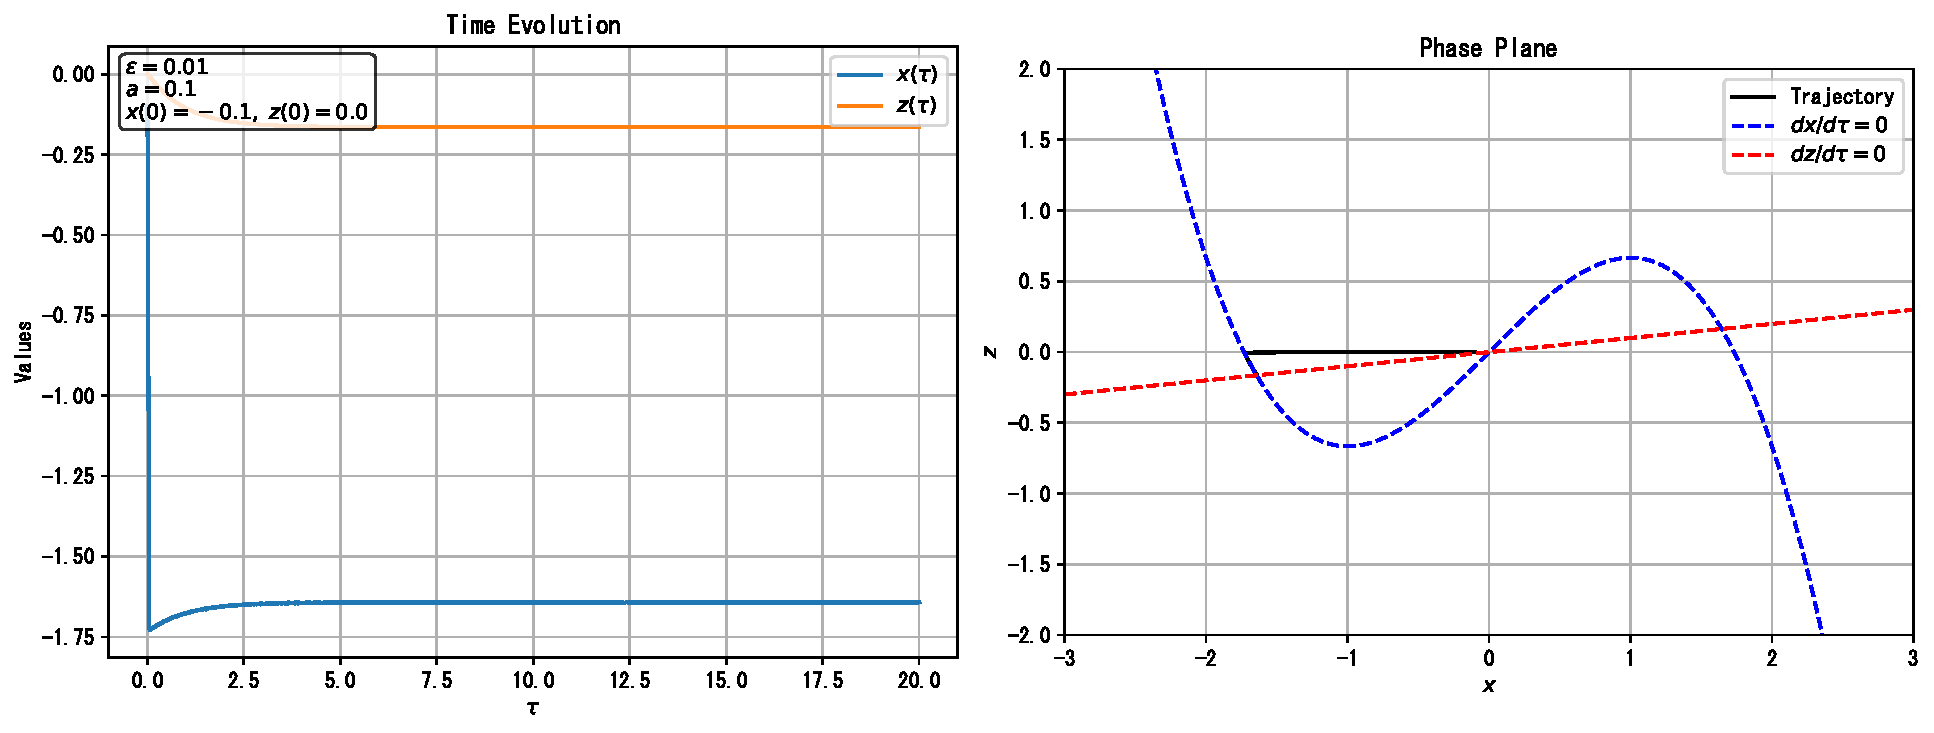
\includegraphics[width=0.98\columnwidth]{plot_1.pdf}
          \caption{a=1.0, \epsilon=0.01,x(0)=-0.1, z(0)=0のときの時間変化と軌跡}
        \end{figure}
        \begin{figure}[H]
          \centering
          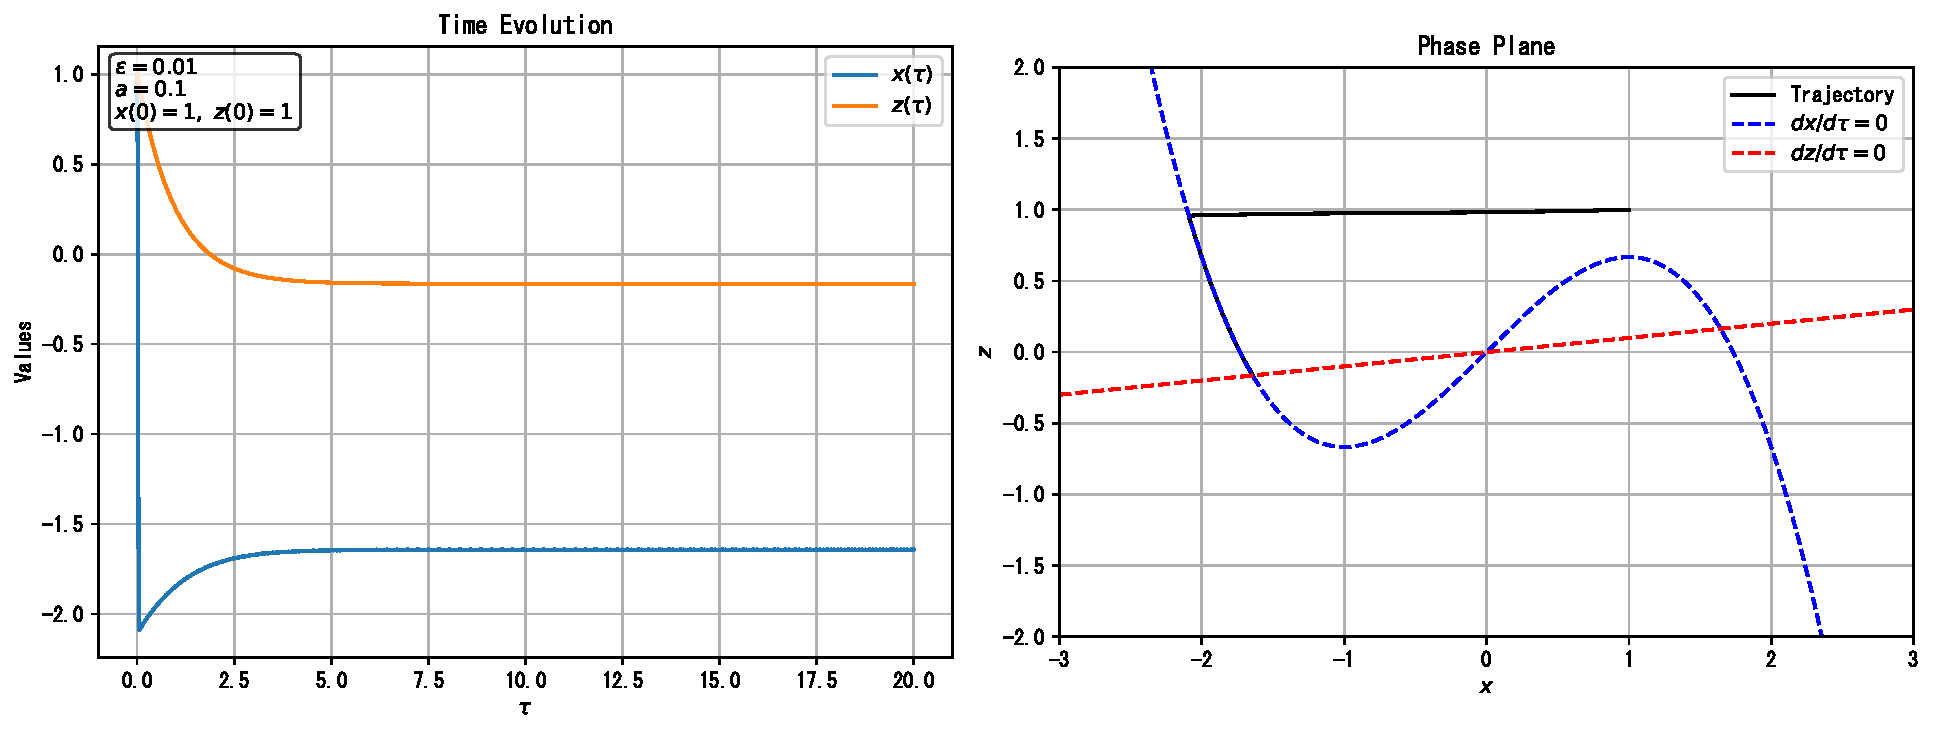
\includegraphics[width=0.98\columnwidth]{plot_2.pdf}
          \caption{a=0.1, \epsilon=0.01,x(0)=1.0, z(0)=1.0のときの時間変化と軌跡}
        \end{figure}
        \begin{figure}[H]
          \centering
          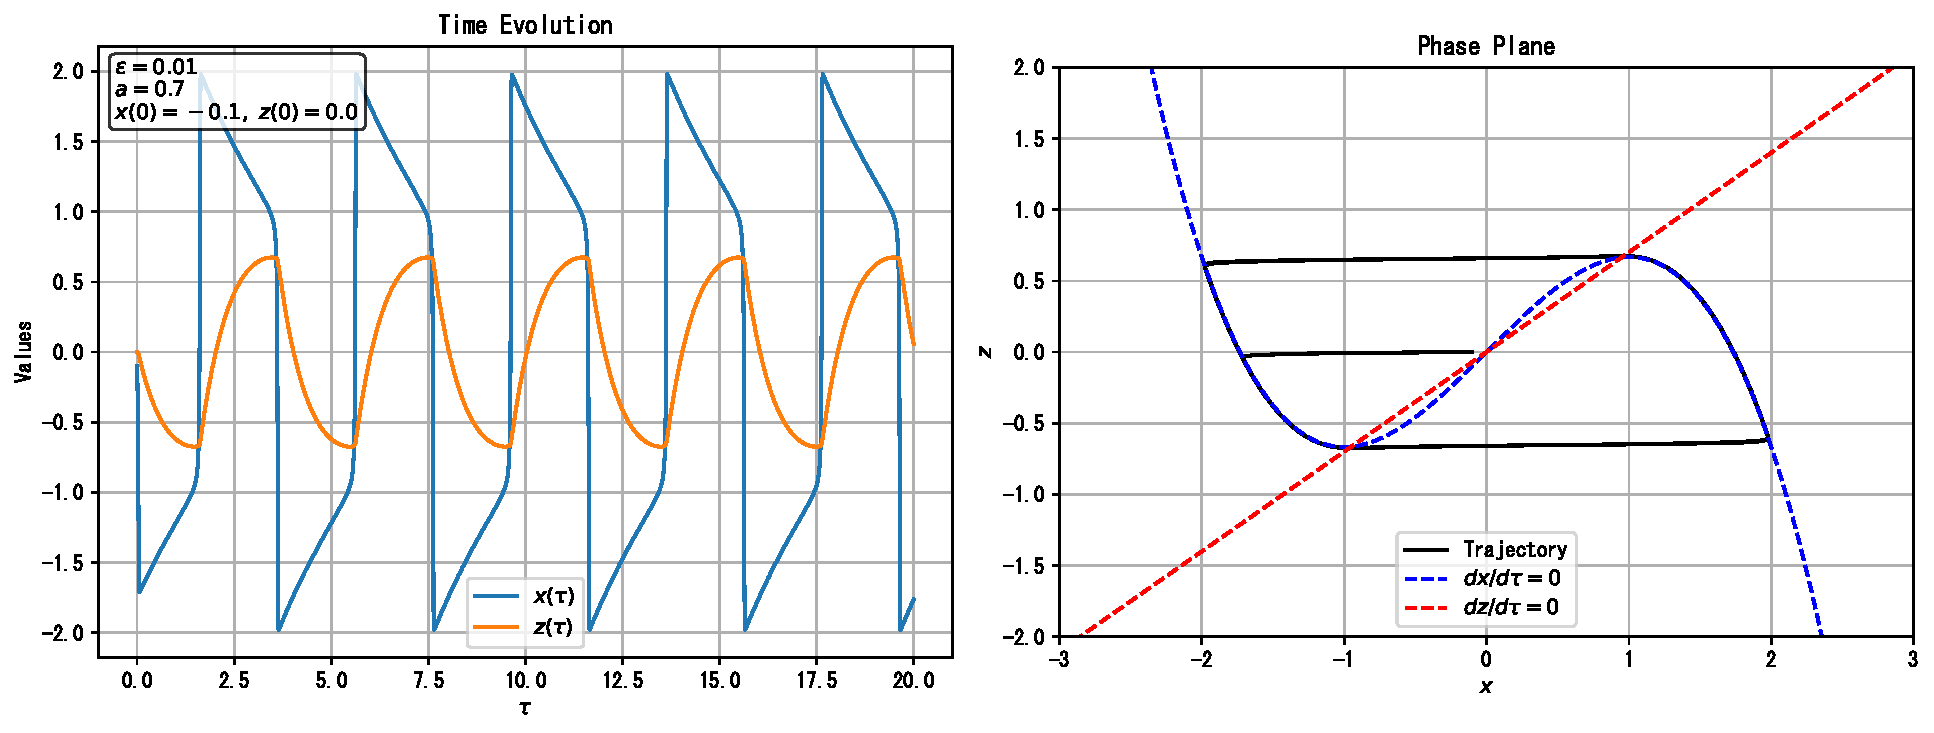
\includegraphics[width=0.98\columnwidth]{plot_3.pdf}
          \caption{a=0.7, \epsilon=0.01,x(0)=-0.1, z(0)=0のときの時間変化と軌跡}
        \end{figure}
        \begin{figure}[H]
          \centering
          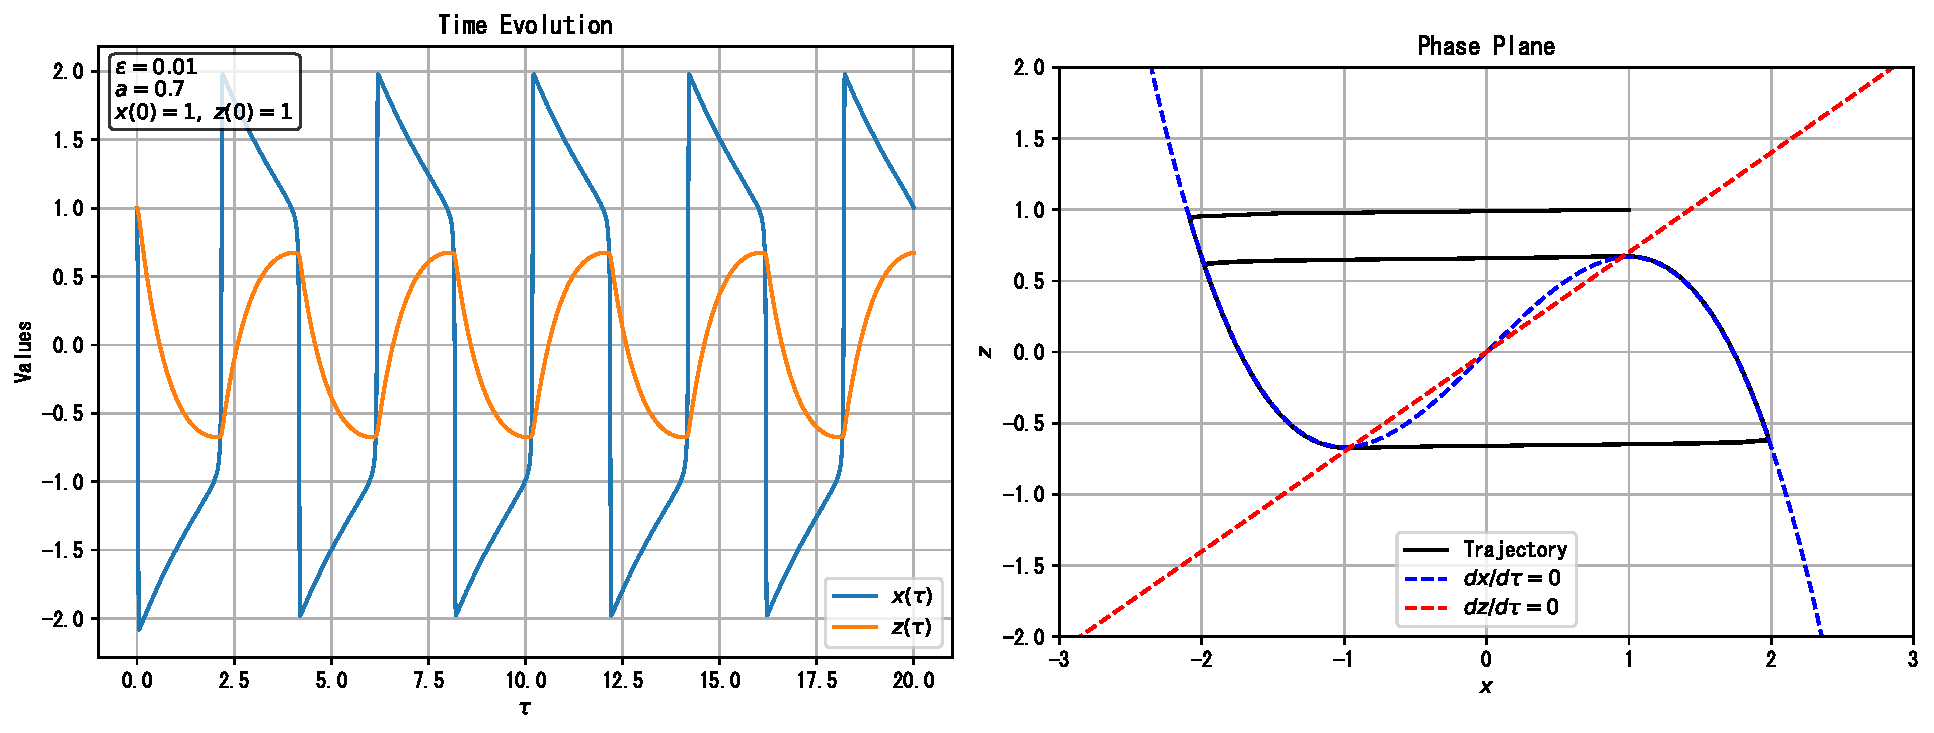
\includegraphics[width=0.98\columnwidth]{plot_4.pdf}
          \caption{a=0.7, \epsilon=0.01,x(0)=1.0, z(0)=1.0のときの時間変化と軌跡}
        \end{figure}
        \begin{figure}[H]
          \centering
          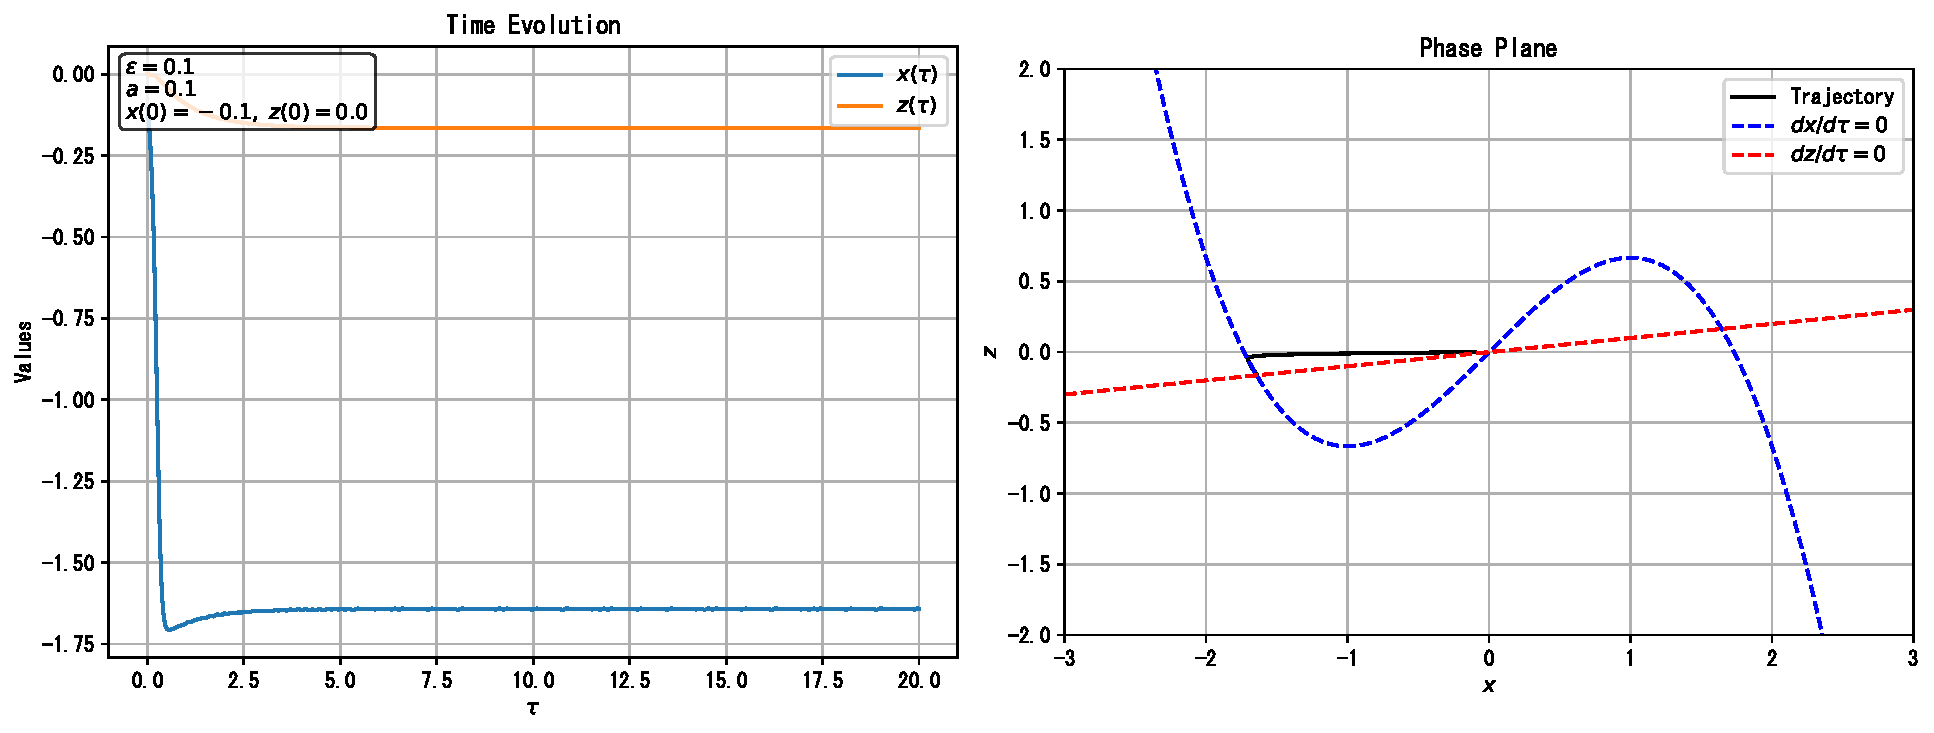
\includegraphics[width=0.98\columnwidth]{plot_5.pdf}
          \caption{a=0.1, \epsilon=0.1,x(0)=-0.1, z(0)=0のときの時間変化と軌跡}
        \end{figure}
        \begin{figure}[H]
          \centering
          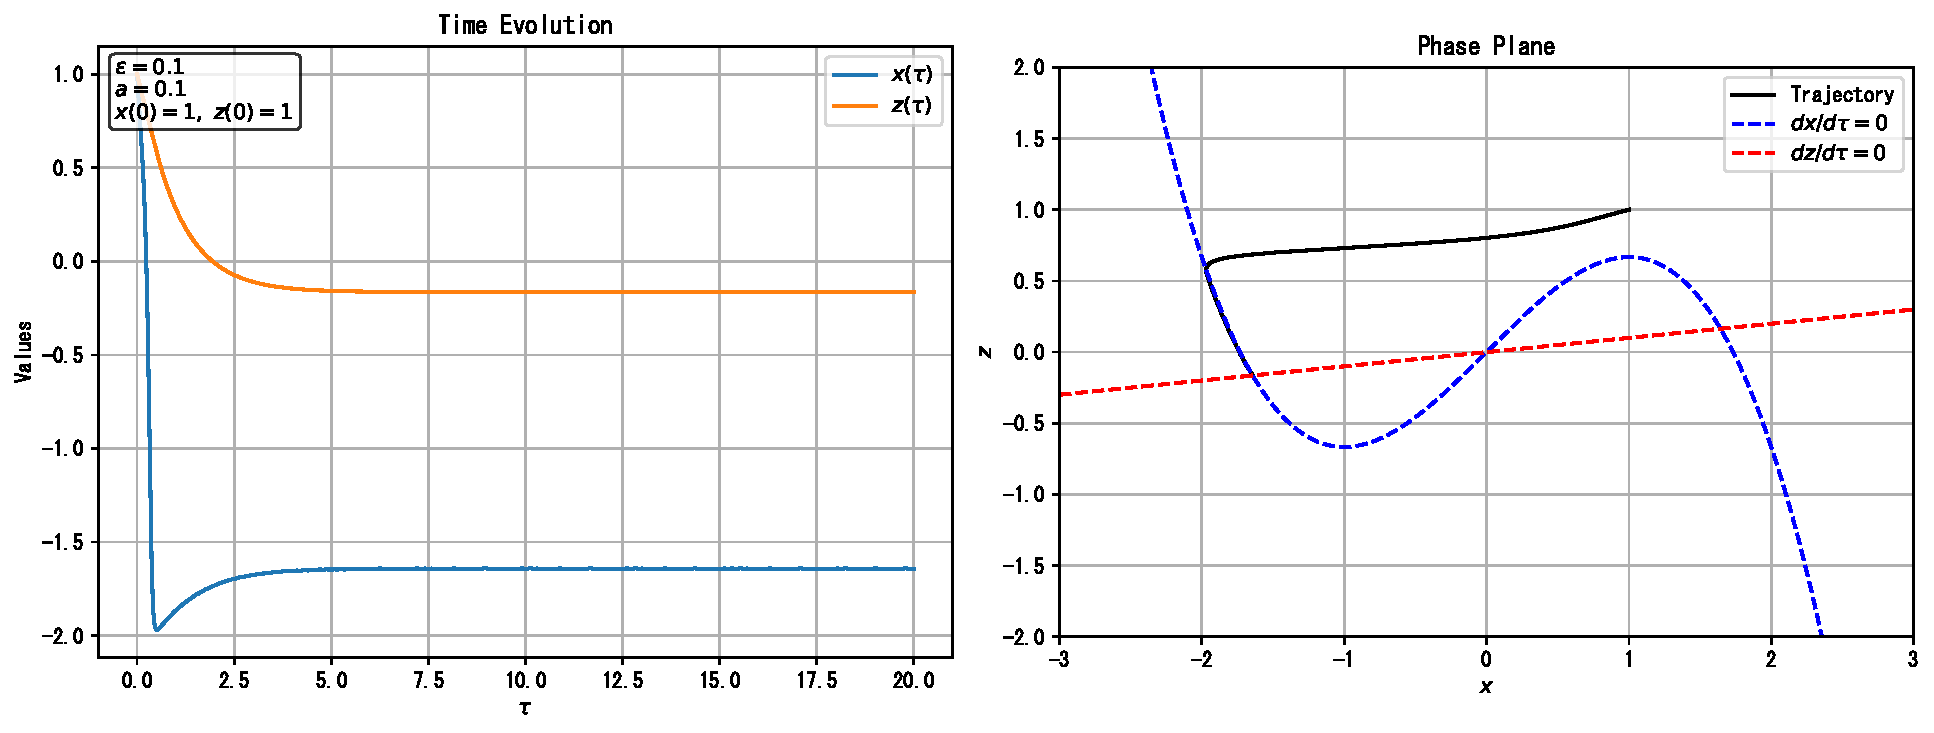
\includegraphics[width=0.98\columnwidth]{plot_6.pdf}
          \caption{a=0.1, \epsilon=0.1,x(0)=1.0, z(0)=1.0のときの時間変化と軌跡}
        \end{figure} 
        \begin{figure}[H]
          \centering
          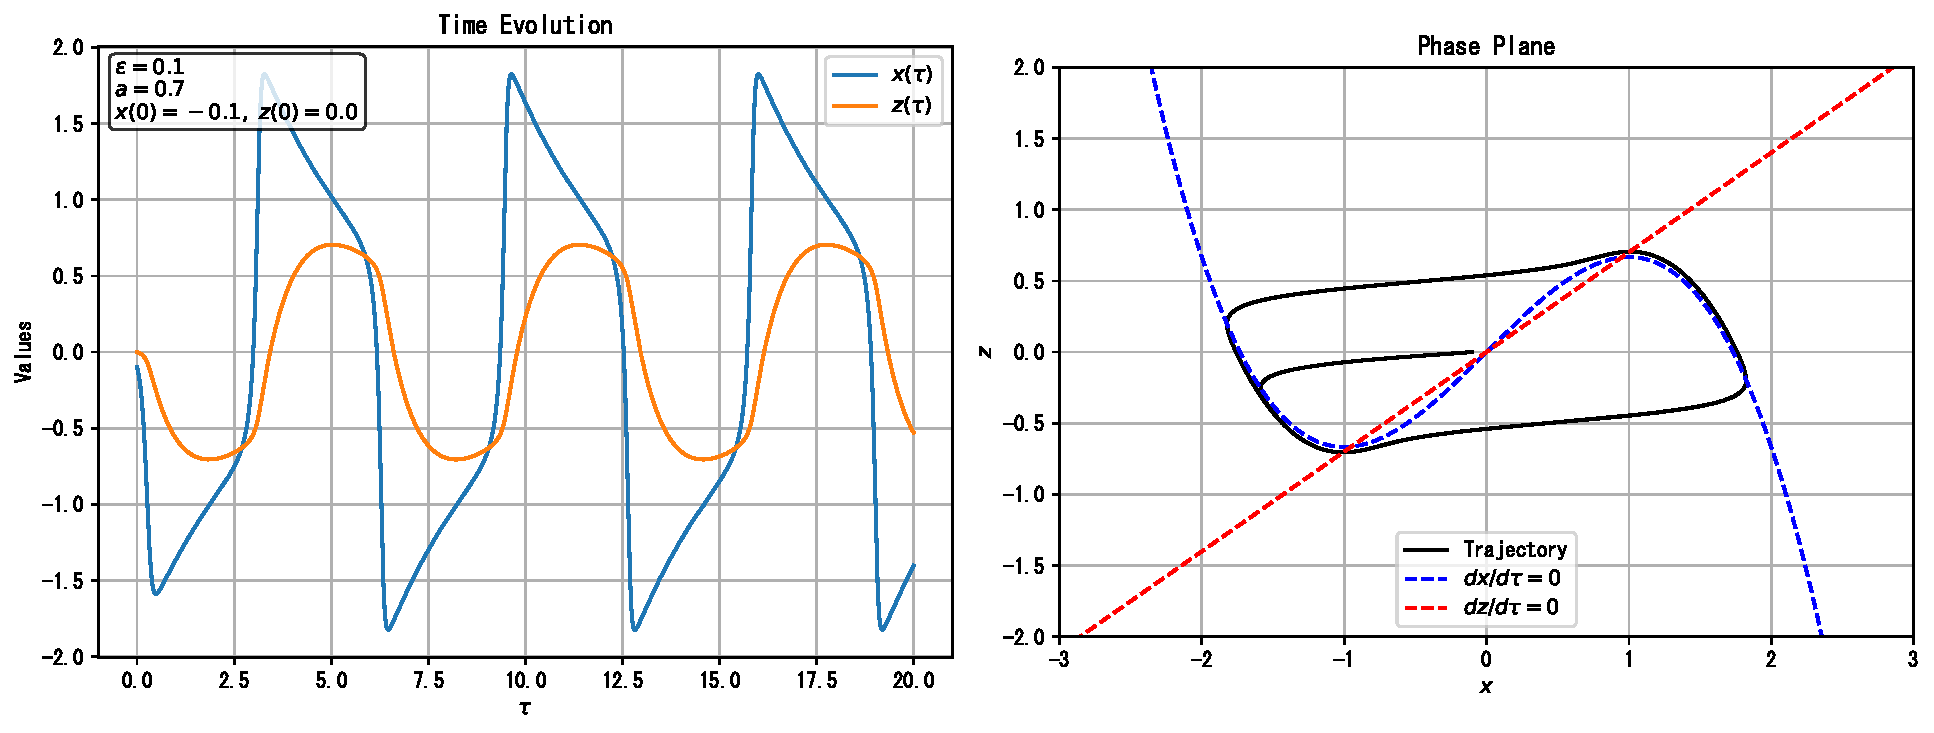
\includegraphics[width=0.98\columnwidth]{plot_7.pdf}
          \caption{a=0.7, \epsilon=0.1,x(0)=-0.1, z(0)=0のときの時間変化と軌跡}
        \end{figure} 
        \begin{figure}[H]
          \centering
          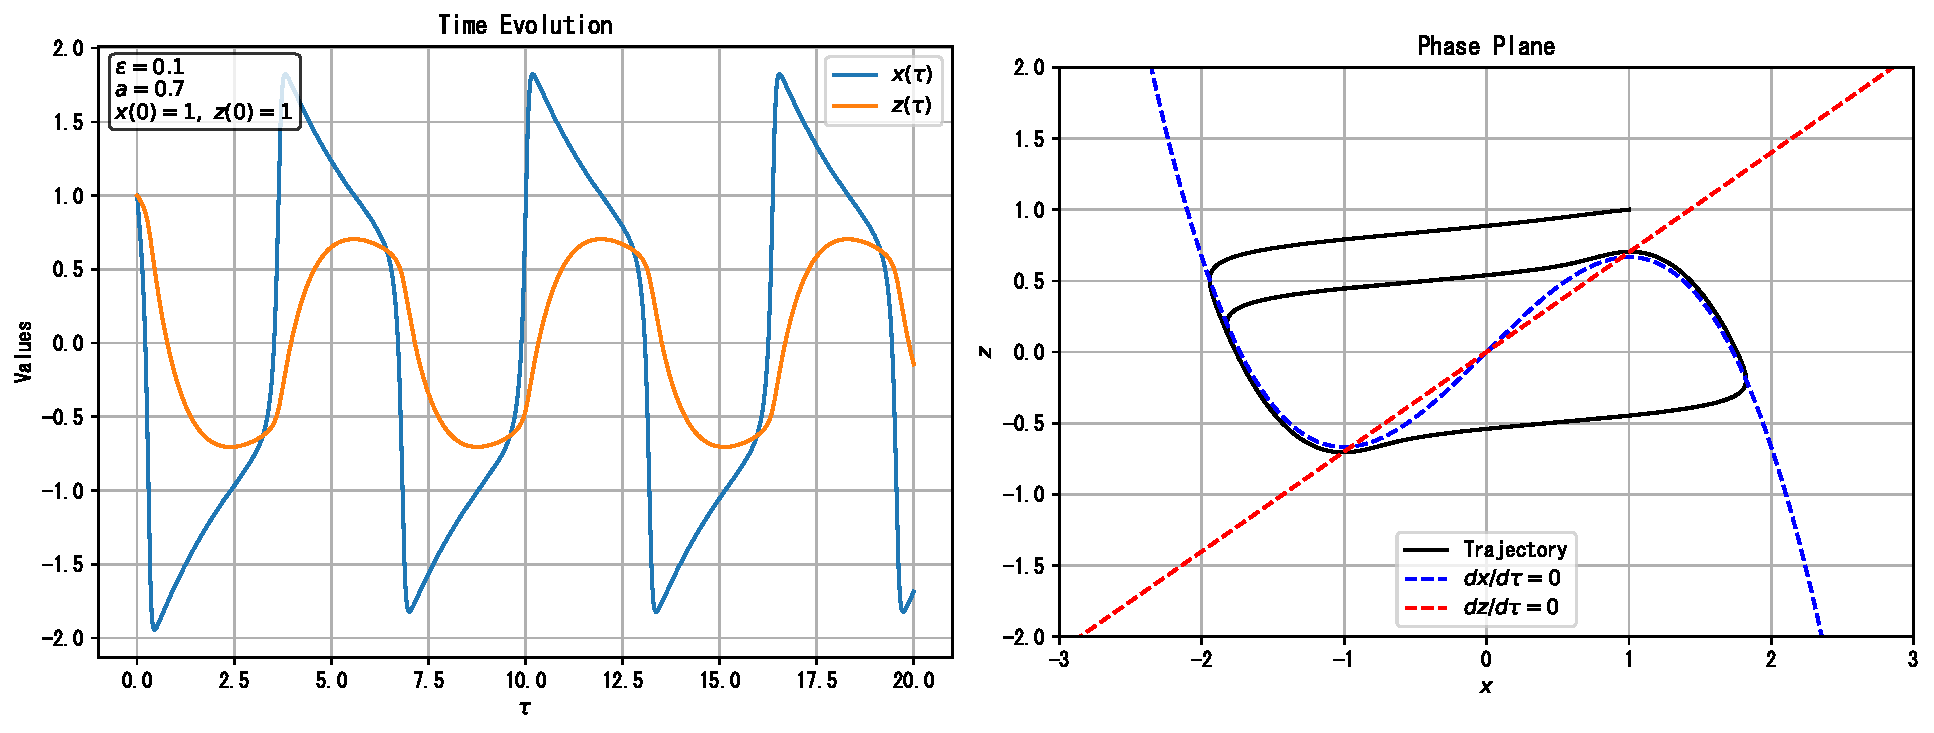
\includegraphics[width=0.98\columnwidth]{plot_8.pdf}
          \caption{a=0.7, \epsilon=0.1,x(0)=1.0, z(0)=1.0のときの時間変化と軌跡}
        \end{figure}
      \subsubsection*{(ii)}
        軌跡はヌルクラインに引き寄せられるような動きを示し, そこを通り過ぎると動きの向きが変化する.
      \subsubsection*{(iii)}
        \epsilon=0に固定し, aを0から1まで0.01刻みで変化させたとき, 安定から振動に変化するaの値を求めた.初期値の影響を考え, ランダムな10個の点を初期値としてx(t)の後半(t=20付近)での最大値と最小値の差がある値を上回っているかを確認し, 初めて上回ったaの値を記録した.(一度振動し始めたものはaを大きくしても再び安定になることはなかった)\\
        その結果, どんな初期値でもa=0.68で振動に変化した.\\
    \section*{発展課題}
      フーリエ解析で有意な周期が得られなかったシャーレのデータをピークを検出し(\cref{fig:peak}), ピーク間距離の平均を周期として求めた.なお,近すぎるピークは除いた.\\
      その結果, 周期はおおよそ0.1754cmであることがわかった.
      \begin{figure}[H]
        \centering
        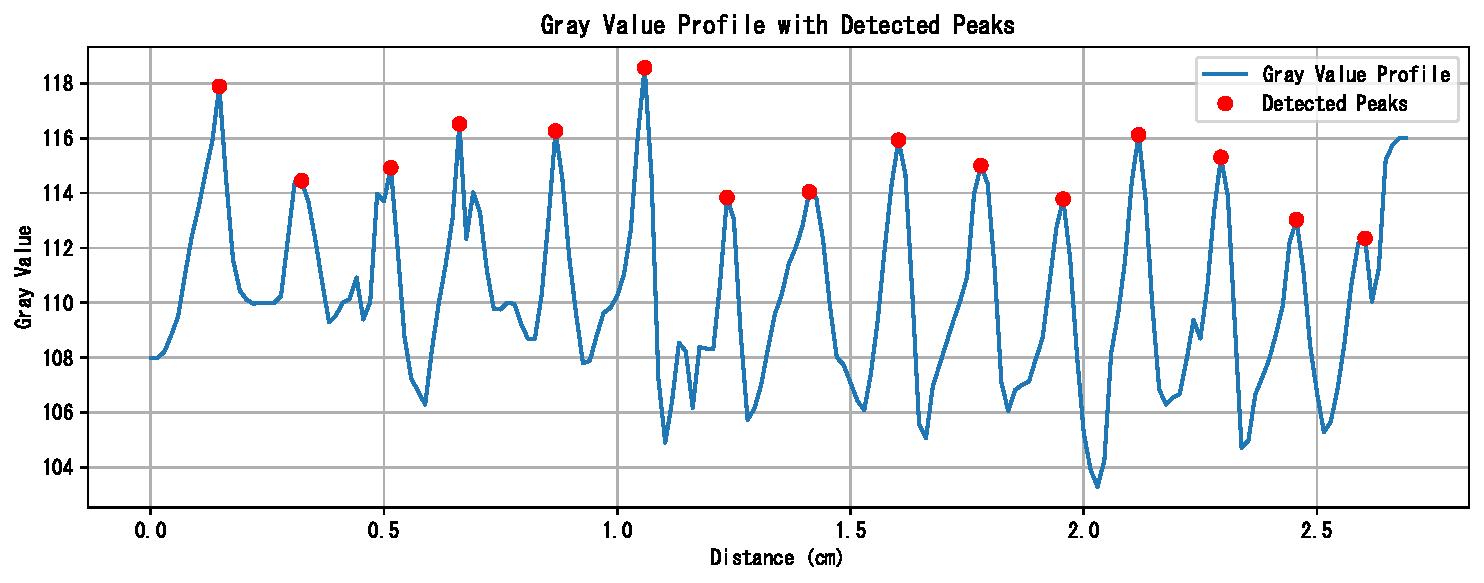
\includegraphics[width=0.7\columnwidth]{prominent_peaks.pdf}
        \caption{ピーク検出したグラフ}
        \label{fig:peak}
      \end{figure}
  \section*{まとめ}
    \noindent BZ反応の原理や反応モデルを理解することができた. \\
    微分方程式を数値的に解く方法を学んだ.
  \section*{参考文献}
    \noindent BZ反応 テキスト\\
    また, データ解析の際のコーディングにchatGPTを用いた.
\end{document}